%=== APPENDIX TABLES ===

\chapter{Appendix Tables and Figures}

\subsection*{Table A-1}

Table \ref{tab:sourceinfo} shows the speaker initials (ID), sex, dialect region number (DR), and the sentences used for each of the sources. Sentences that are trimmed are denoted with asterisks. 

\begin{table}[!htp]
    \footnotesize\centering
    \begin{tabularx}{\textwidth}{clccLLLL}
\toprule
Source & Speaker ID & Sex & DR & Sentences\\
\midrule
1 & JWT0 & M & 1 & SI1291& SI751& SI1381*\\
2 & AEM0 & F & 2 & SA1& SA2& SI762& SI1392*\\
3 & SLS0 & F & 3 & SI1056& SI1686& SI2316\\
4 & BAS0 & F & 4 & SI1387& SI1472& SI2066*\\
5 & DWH0 & M & 5 & SI1168& SI1925& SX35\\
6 & JRK0 & M & 6 & SI1662& SI2130& SI880& SX160*\\
\bottomrule
\end{tabularx}
    \caption[Speaker information for the evaluation sources]{Speaker information for the evaluation sources\\
    \footnotesize{M - male; F - female. DR1 - New England; DR2 - Northern; DR3 - North Midland; DR4 - South Midland; DR5 - Southern; DR6 - New York City.}}
    \label{tab:sourceinfo}
\end{table}

\subsection*{Table A-2}

\begin{table}[!htp]
    \footnotesize\centering
    \begin{tabularx}{\textwidth}{cL}
\toprule
Source & Transcript\\
\midrule
1 & they should live in modest circumstances avoiding all conspicuous consumption serve in frankfurter buns or as a meat dish but briefly the topping \\
2 & 
she had your dark suit in greasy wash water all year
don't ask me to carry an oily rag like that
fill small hole in bowl with clay 
assume for\\
3 & can thermonuclear war be set off by accident it latches when you close it so stay as long as you like Davy Mathews it's disgusting the way you're always eating\\
4 & several factors contributed to this change she greeted her husband's colleagues with smiling politeness offering nothing He saw a pint-sized man\\
5 & it takes a great deal of sophisticated thought to get the impact of this fact so what's this all about help celebrate your brother's success\\
6 & did anyone see my cab See you in about an hour the revolution now under way in materials handling makes this much easier as co-authors we presented our new book\\
\bottomrule
\end{tabularx}
    \caption{Transcript of the evaluation sources}
    \label{tab:transcript}
\end{table}
\newpage %ADD NEW PAGE

\subsection*{Figure A-1}

\begin{figure}[!htb]
    \centering
    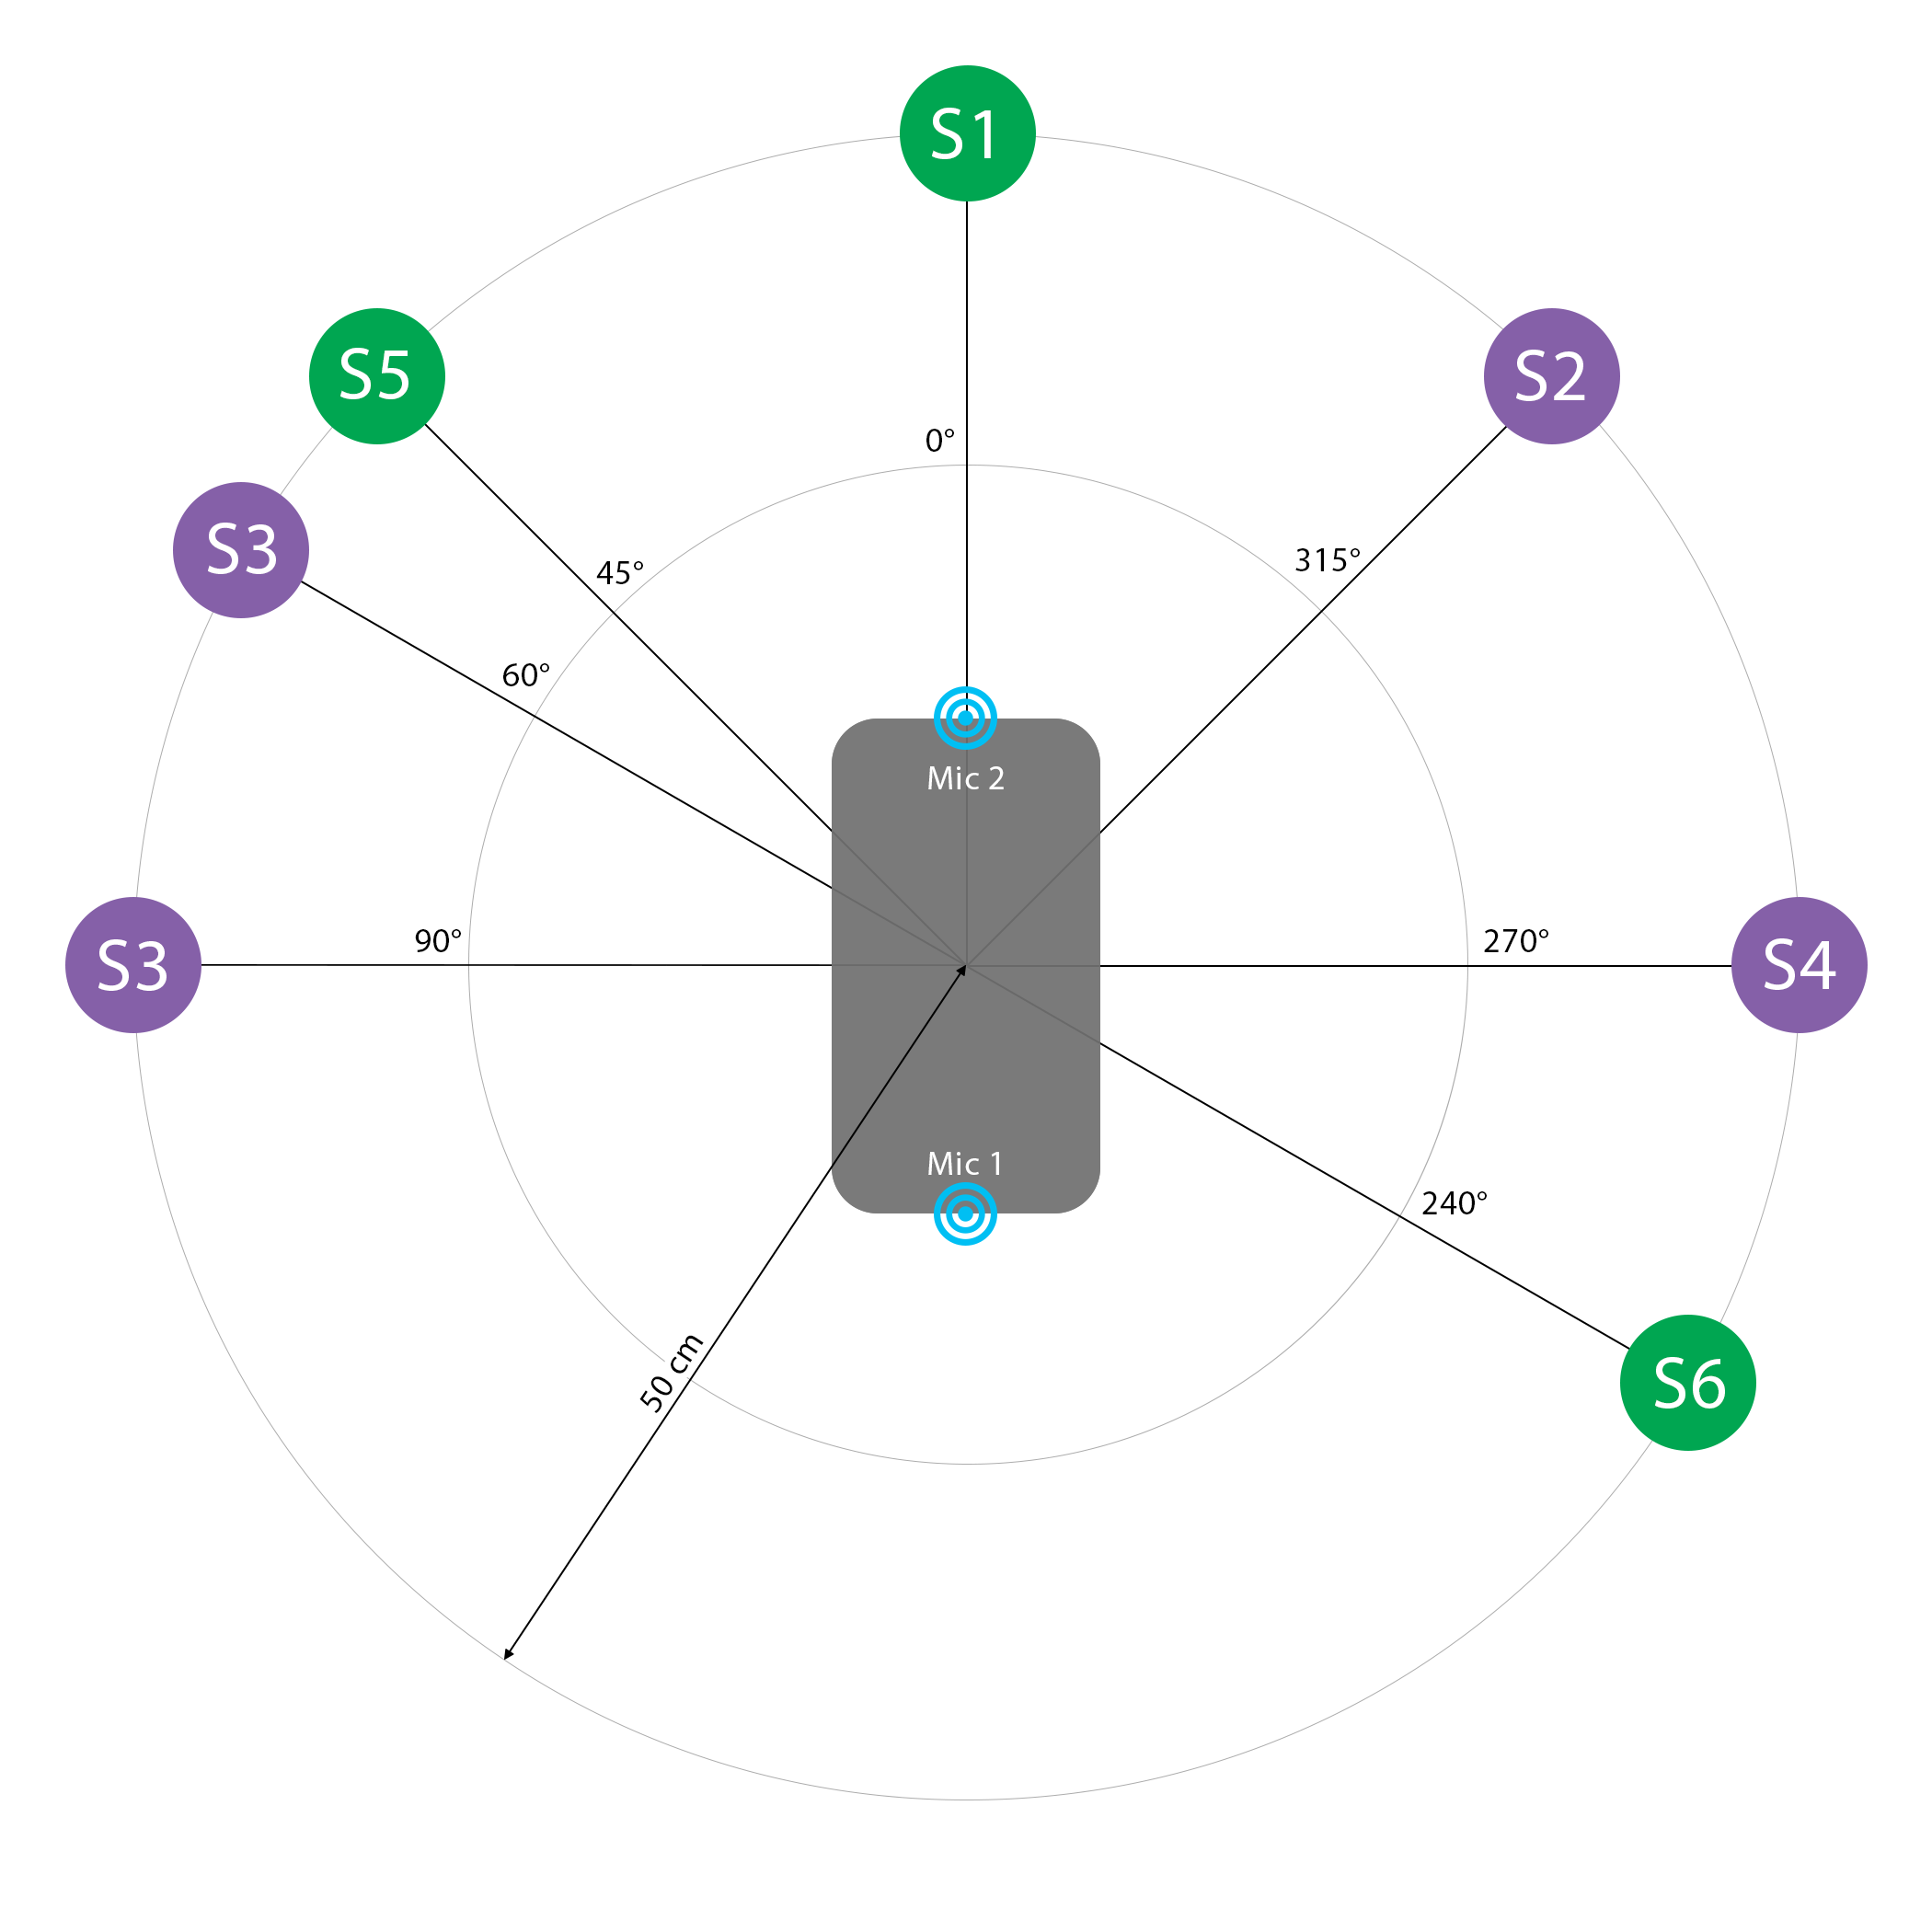
\includegraphics[width = 0.9\textwidth]{fig/sourcelocation.png}
    \caption[Positions of the loudspeaker for each source speaker]{Positions of the loudspeaker for each source speaker \\\footnotesize{A green circle denotes a male speaker. A purple circle denotes a female speaker. The angle is measured with respect to the line passing through the microphones in a counterclockwise manner, starting from the top of the phone where Microphone 2 is located. Note that Speaker 3 was recorded at two different positions. The figure is not to scale.}}
    \label{fig:anglesummary}
\end{figure}

\FloatBarrier

\subsection*{Figures A-2 - A5}

The configurations of the mixtures are shown, not to scale, in Figures \ref{fig:2mix1} to \ref{fig:3mix2}. The source configuration for each mixture is the same across all acoustic environments.\newpage

\vspace*{-3.9em}\noindent
\begin{minipage}{\linewidth}\noindent
\begin{multicols}{2}
\begin{Figure}
    \centering
    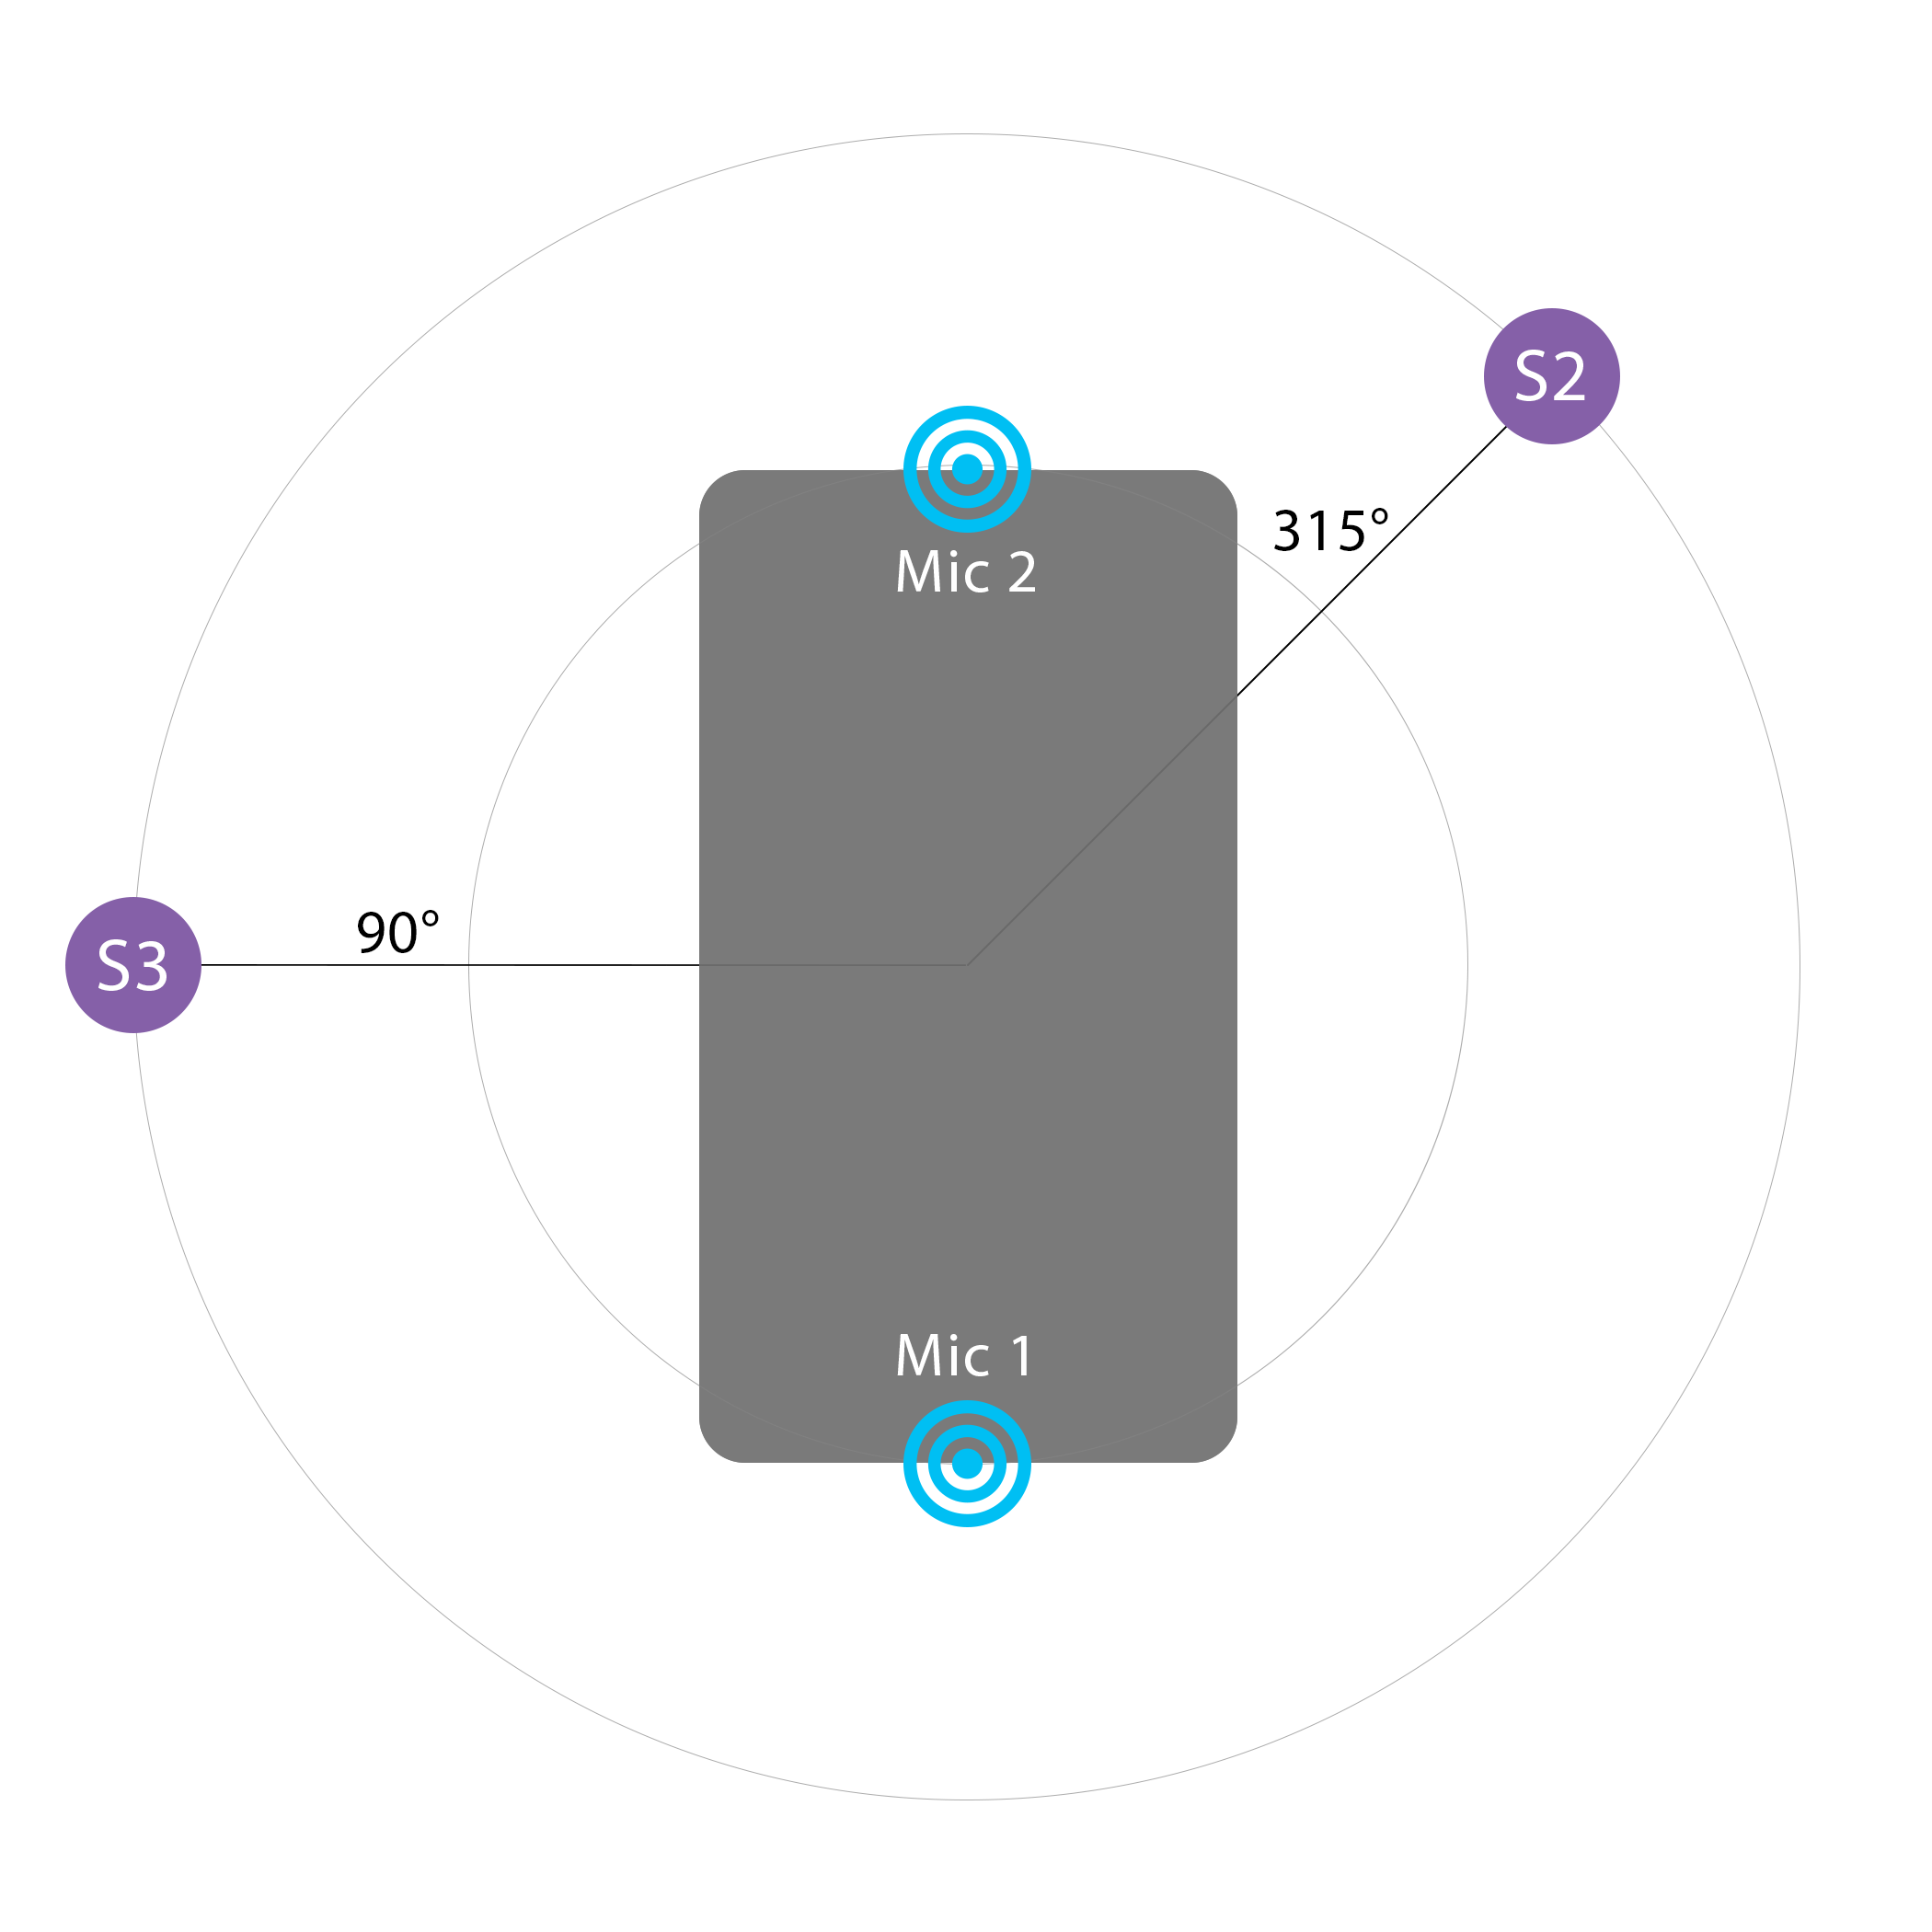
\includegraphics[width=0.99\linewidth]{fig/2mix1.png}
    \captionof{figure}{Configuration 1 for two-source mixture}
    \label{fig:2mix1}
\end{Figure}
\begin{Figure}
    \centering
    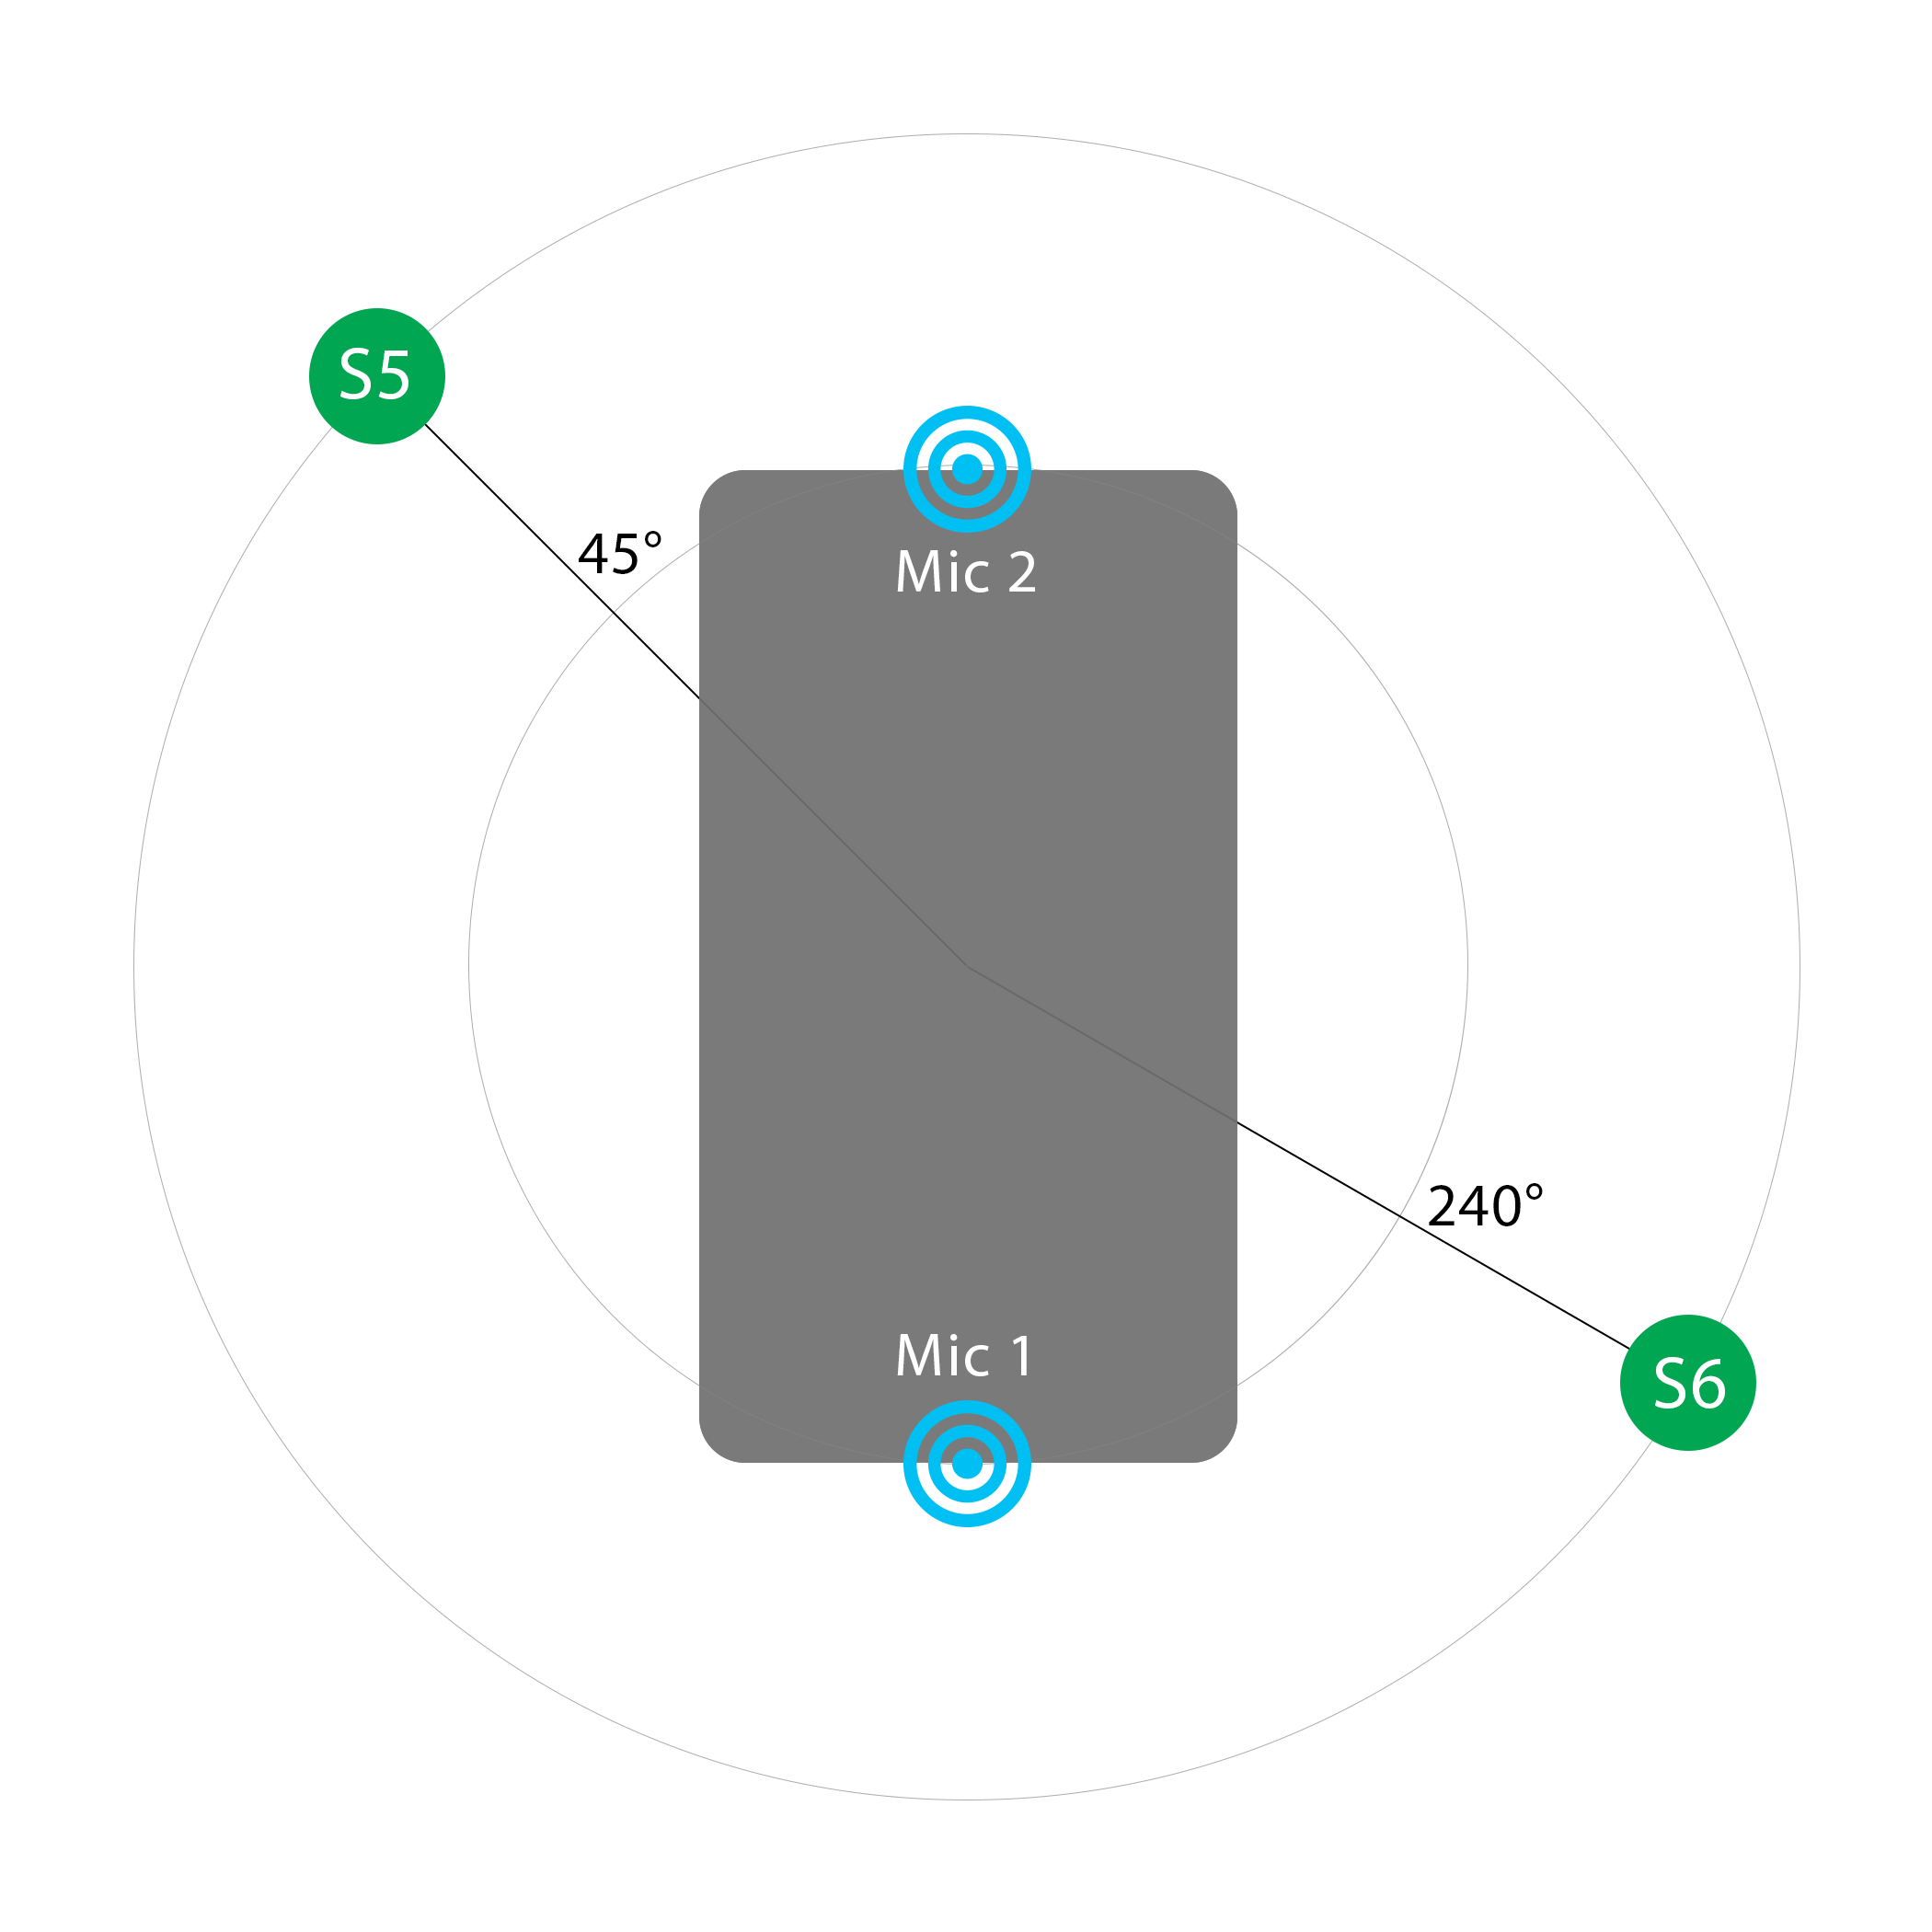
\includegraphics[width=0.99\linewidth]{fig/2mix2.png}
    \captionof{figure}{Configuration 2 for two-source mixture}
    \label{fig:2mix2}
\end{Figure}
\begin{Figure}
    \centering
    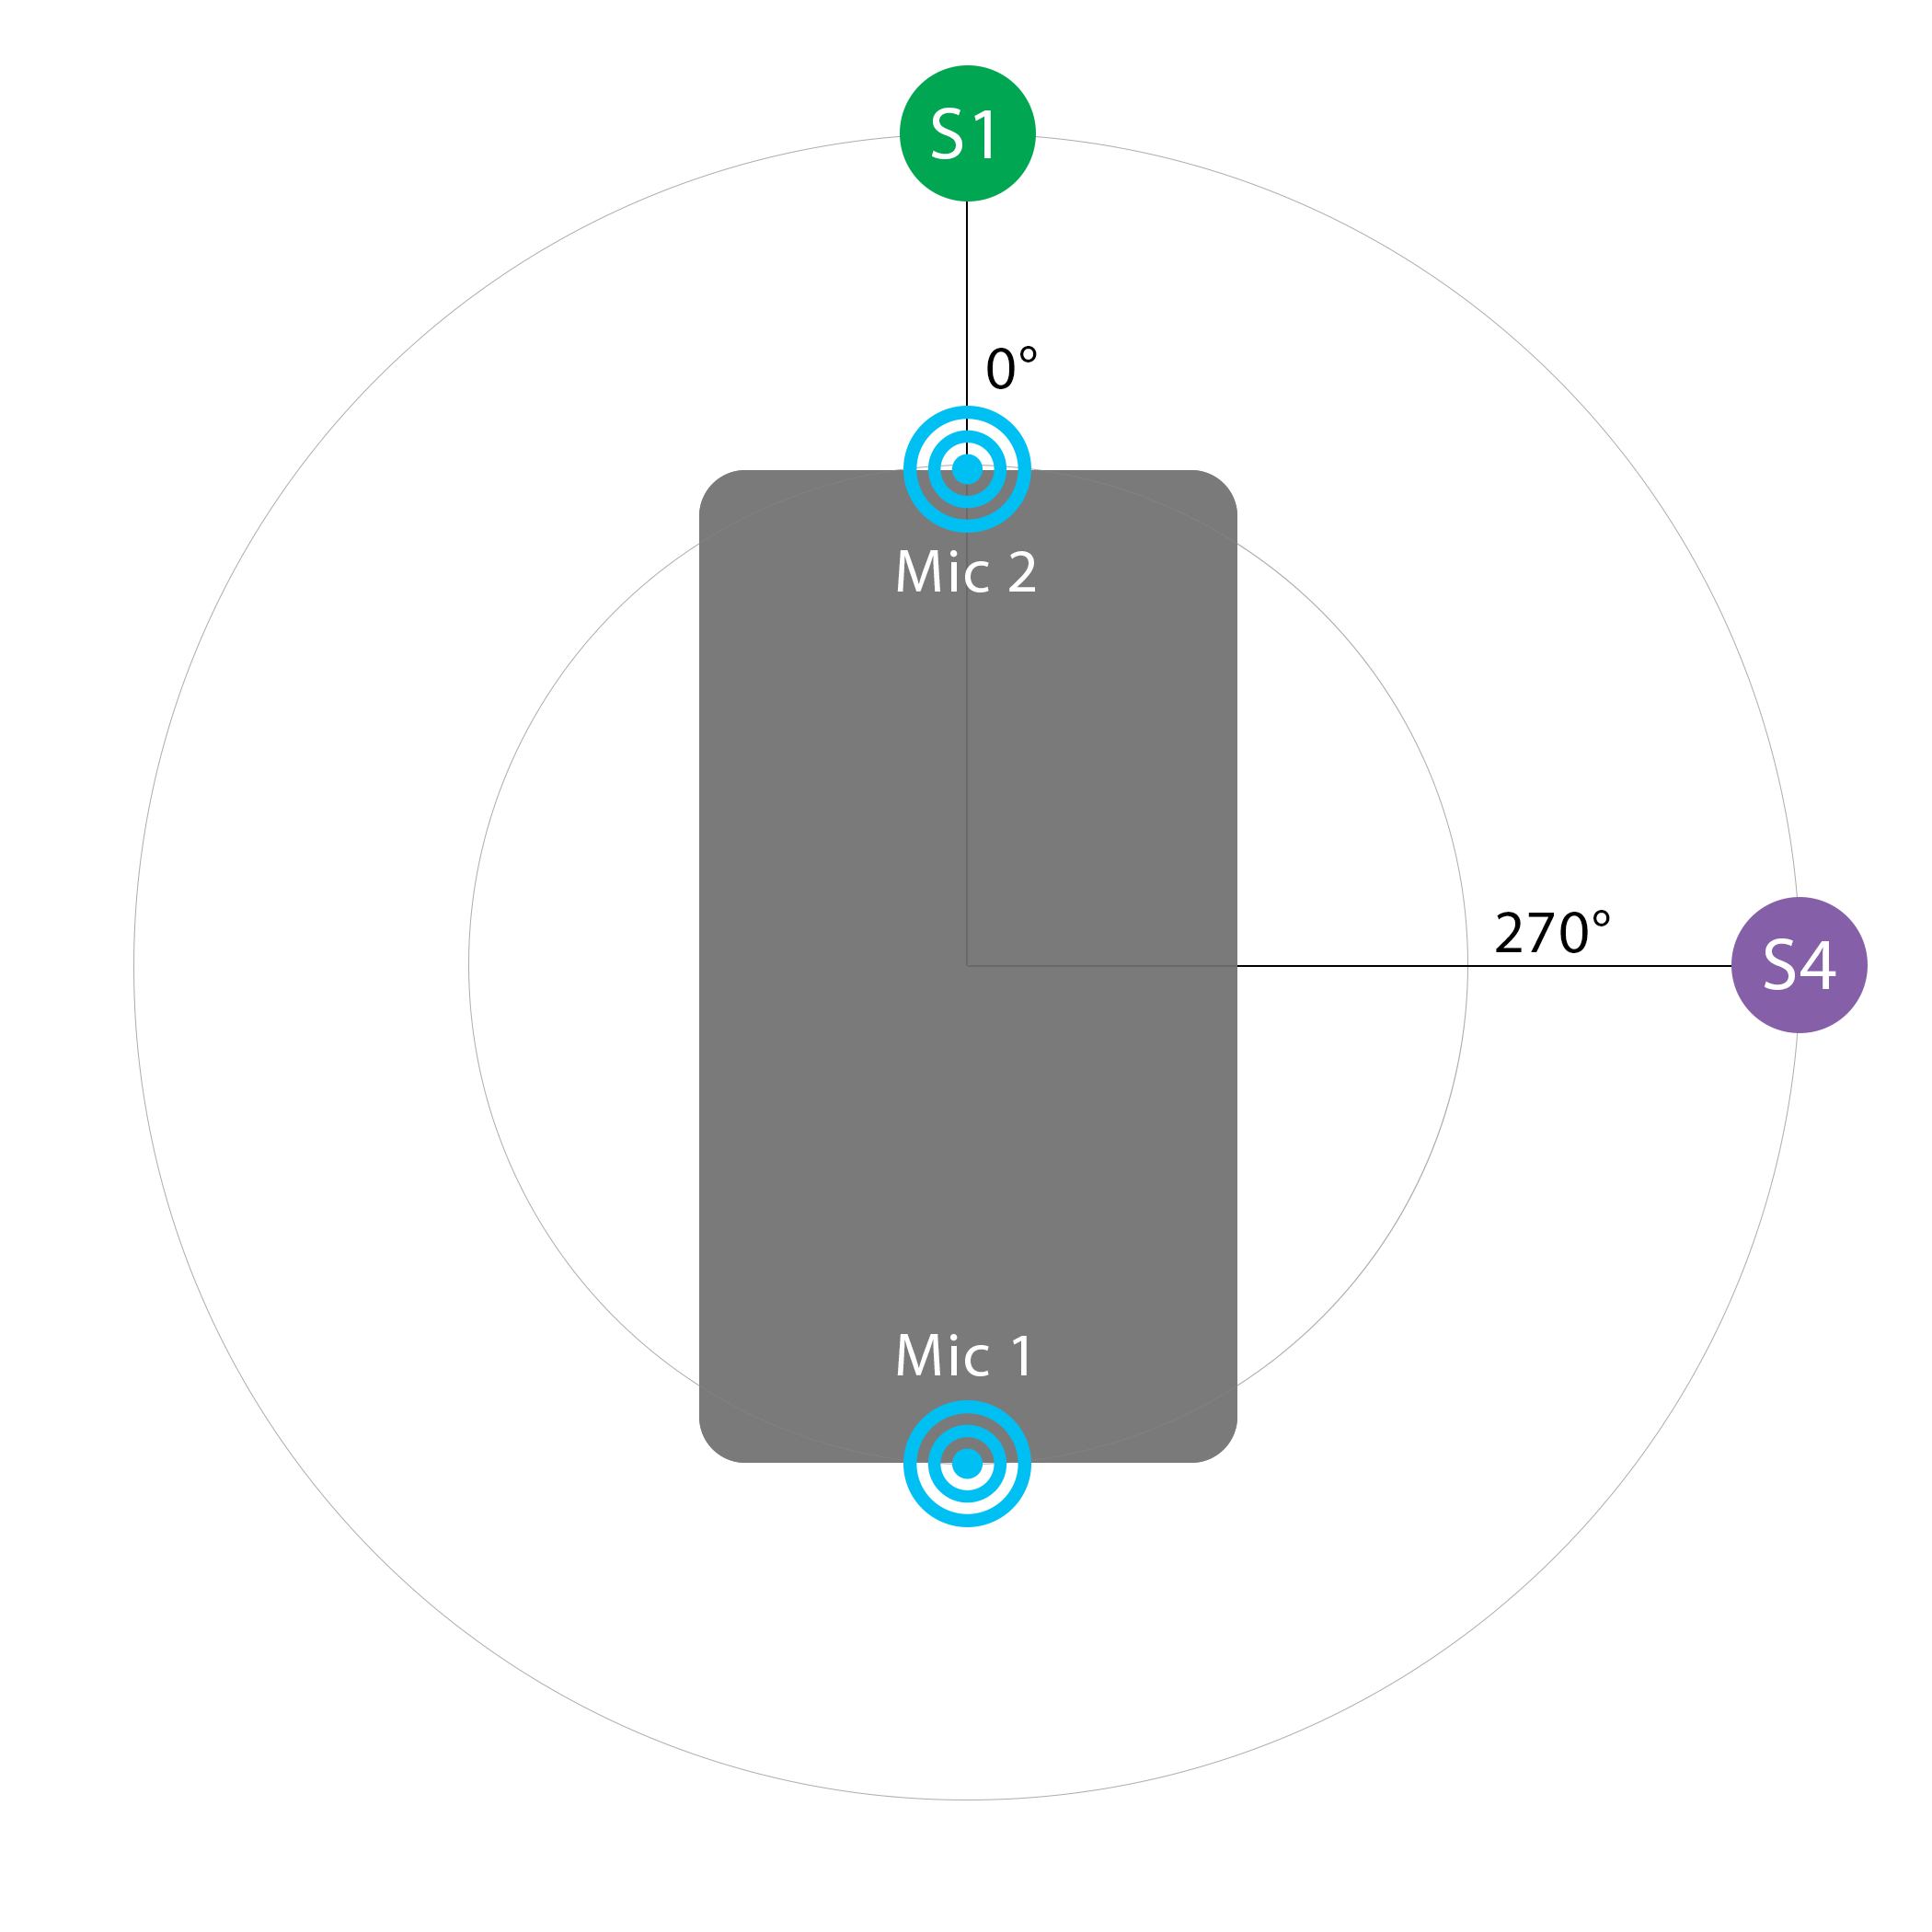
\includegraphics[width=0.99\linewidth]{fig/2mix3.png}
    \captionof{figure}{Configuration 1 for three-source mixture}
    \label{fig:3mix1}
\end{Figure}
\begin{Figure}
    \centering
    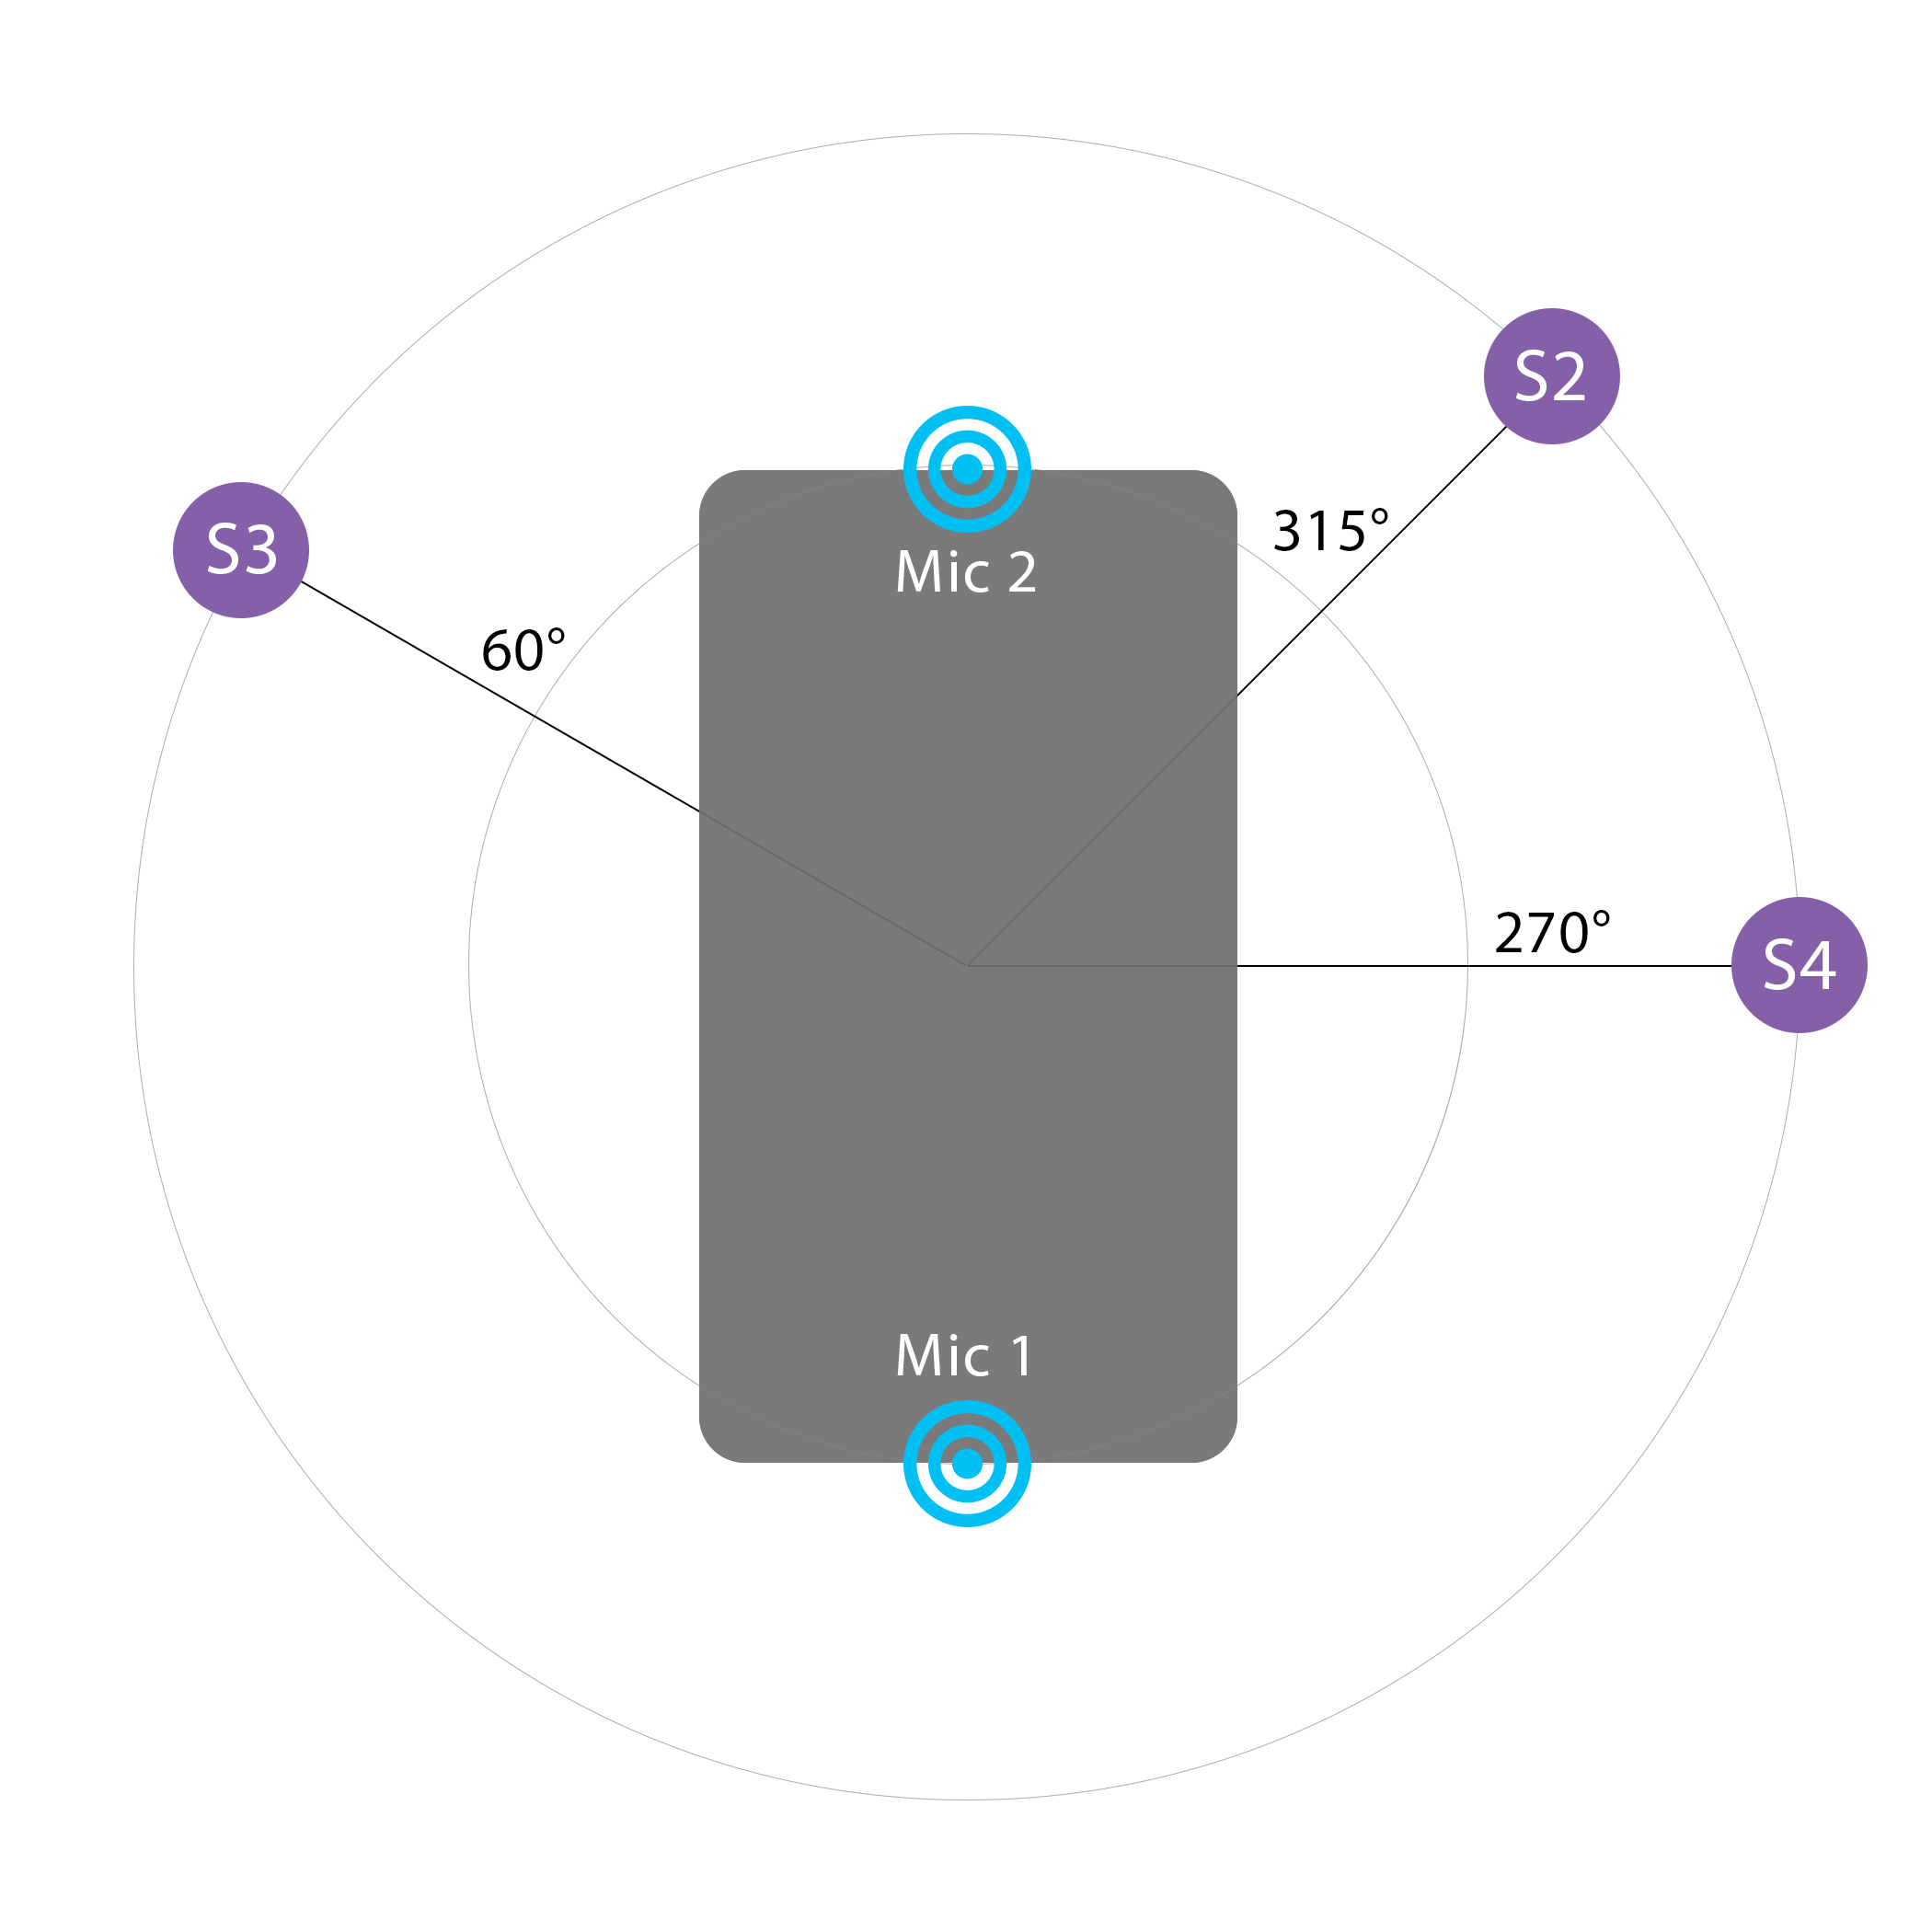
\includegraphics[width=0.99\linewidth]{fig/3mix1.png}
    \captionof{figure}{Configuration 2 for three-source mixture}
    \label{fig:3mix2}
\end{Figure}
\end{multicols}
\end{minipage}
\vfill






%=== END OF APPENDIX TABLES AND FIGURES===
\newpage
